\documentclass[15pt]{extarticle}
\usepackage{cs}

\begin{document} 
\fontsize{12pt}{12pt}\selectfont
\thispagestyle{empty}
\section*{演算法設計方法論(Design Strategies for Computer Algorithms) \\
\normalsize{Homework 4} \\
\normalsize{DUE DATE: JANUARY 8, 2018}}

\hfill \textbf{學號:b03902129 \, 系級:資工四 \, 姓名:陳鵬宇} \\

% 1
\section{問題定義}

\vskip3mm
\textbf{問題}:\begin{minipage}[t]{0.8\linewidth}
    \textit{Determining whether a point belongs to the union of given $n$ circles} \vskip0mm
\end{minipage}
\vskip3mm
\textbf{輸入}:
\begin{minipage}[t]{0.8\linewidth}
\begin{itemize}
    \item $n$ 個圓$C_i(Q_i,r_i)$,其中圓心座標 $Q_i(x_i,y_i)$ 且半徑 $r_i$。
    \item 一點 $P(x,y)$
\end{itemize}
\end{minipage}

\vskip3mm
\textbf{輸出}:
\begin{minipage}[t]{0.8\linewidth}
    \begin{itemize}
        \item \textbf{TRUE}, $P\in C_i,\forall i$
        \item \textbf{FALSE}, $P\notin C_i,\forall i$
    \end{itemize}
\end{minipage}


% 2
\section{解法敘述}
% 2.1
\subsection{The Algorithm of Shamos and Hoey}

給定一$n$個點的集合$S=\{P_1,P_2,\dots,P_n\}$
\begin{enumerate}
    \item 根據$x$座標對這$n$個點排序
    \item 給予新的座標
    \item 將$S$分成兩個子集$L=\{P_1,P_2,\dots,P_{[n/2]}\}$和$R=\{P_{[n/2]+1},P_{[n/2]+2},\dots,P_n\}$
    \item 分別對$L$和$R$中的點建構沃羅諾伊圖$V(L)$和$V(R)$
    \begin{itemize}
        \item 分治線(Dividing line)使得 $L(R)$ 中的每一點都會更靠近他們原本的那一側$L(R)$。
        \item 時間複雜度:$O(n)$。
    \end{itemize}
\end{enumerate}

\begin{lemma}
    分治線由延伸至無窮的兩條射線和一些有限的線段組成。每一個元素(一射線或一線段)包含於$V(L)$中$V(P_i)$和$V(R)$中$V(P_j)$相交的部分,其中$P_i\in L, P_j\in R$且會是$P_i$和$P_j$的垂直平分線。
\end{lemma}

\begin{lemma}
    每兩條射線必定是凸包CH$(S)$連續兩點的垂直平分線,其中一條位於$L$,另一條位於$R$。
\end{lemma}

Lemma 1 告訴我們可以在 $O(n)$ 內找到分治線 。\\

Lemma 2 告訴我們可以在 $O(n)$ 內在 CH$(S)$找到所述射線,同時可在$O(n)$內分別從CH$(L)$和CH$(R)$找到一條射線。

\subsection{建構沃羅諾伊圖}
\begin{enumerate}
    \item 將$n$個圓 $C_i(Q_i,r_i)$分為兩子集 \\
        根據 2.1 Shamos 和 Hoey 所提出的演算法,我們可以以得到兩個沃羅諾伊圖$V(L)$和$V(R)$。
        \begin{center}
            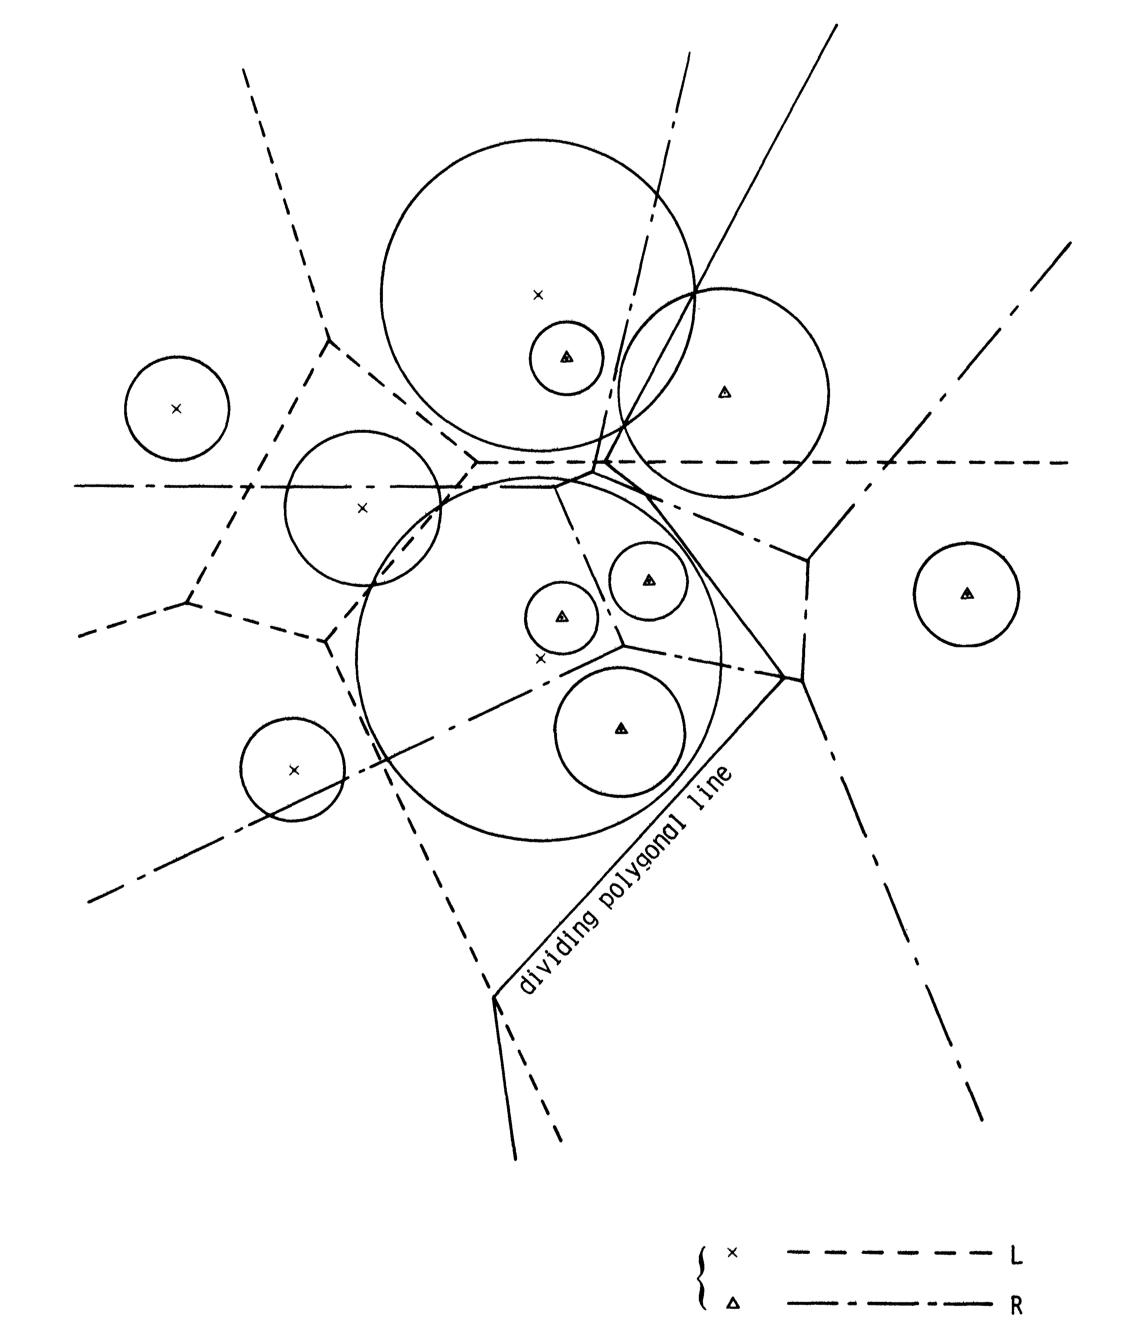
\includegraphics[width=0.5\textwidth]{fig4.png}
        \end{center}
    \begin{lemma}
        分治線是單行的,由兩條射線和幾條有限線段組成。Laguerre幾何中的巨觀下,多邊型左邊(右邊)的每一點與$L(R)$中的某個圓比$R(L)$中的任何圓更接近。
    \end{lemma}

    \item 在$O(n)$內找到分治線 \\
    利用沃羅諾伊邊皆為直線的性質,便可以順時針方向掃描在$O(n)$內找到分治線。

    \item 在$O(n)$內找到射線 \\
    凸包邊緣可能退化至一直線,而有些情況會變得不成立。
    \begin{center}
        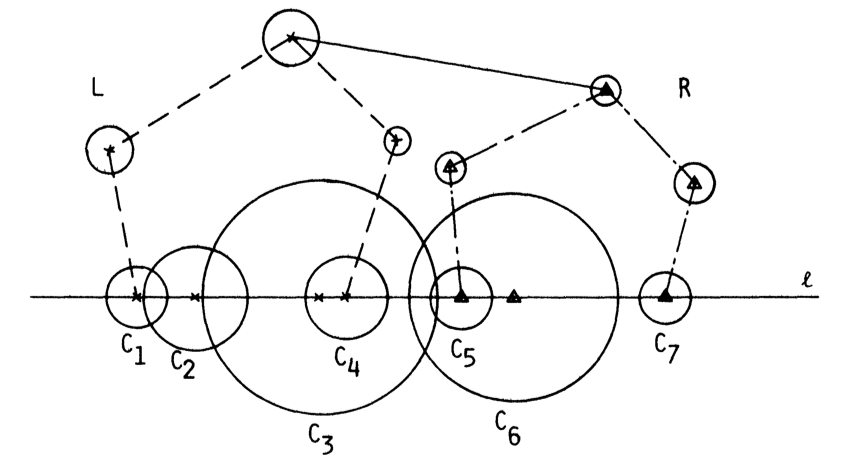
\includegraphics[width=0.5\textwidth]{fig5.png}
        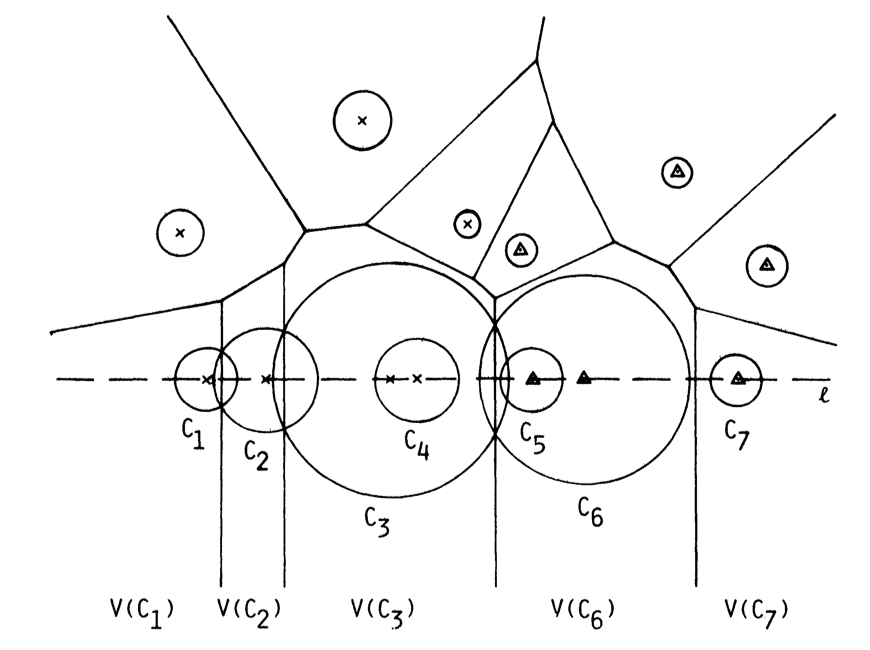
\includegraphics[width=0.5\textwidth]{fig6.png}
        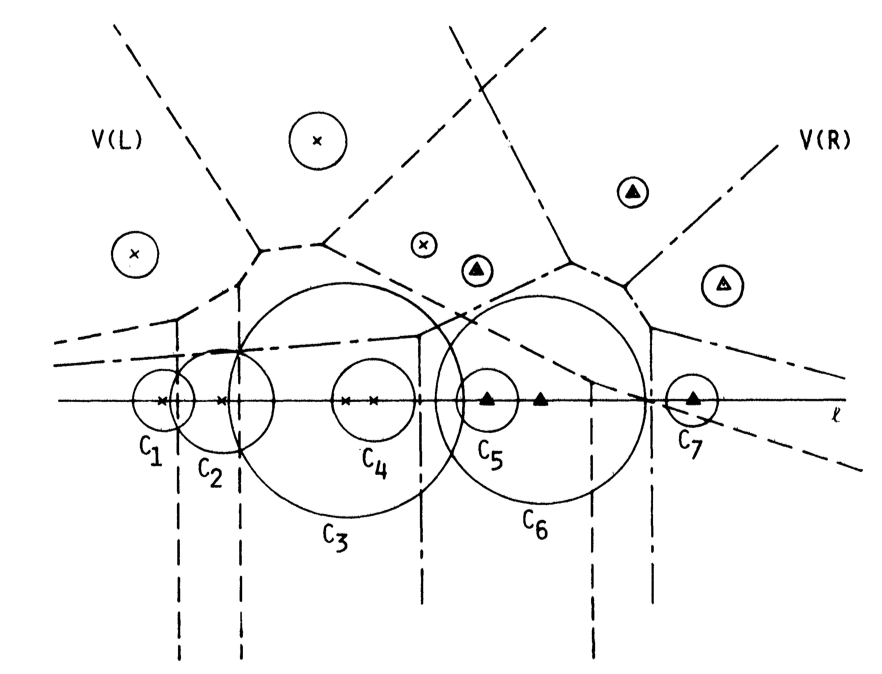
\includegraphics[width=0.5\textwidth]{fig7.png}
    \end{center}
    由於在$V(L_l)$和$V(R_l)$中所有沃羅諾伊邊都與直線$l$,所以我們可以在$O(n)$內合併$V(L_l)$和$V(R_l)$來
    得到$V(L_l\cap R_l)$。由於在沃羅諾伊圖中區域數量的複雜度為$O(n)$,因此可以在$O(n)$內找到分治線。
    \begin{center}
        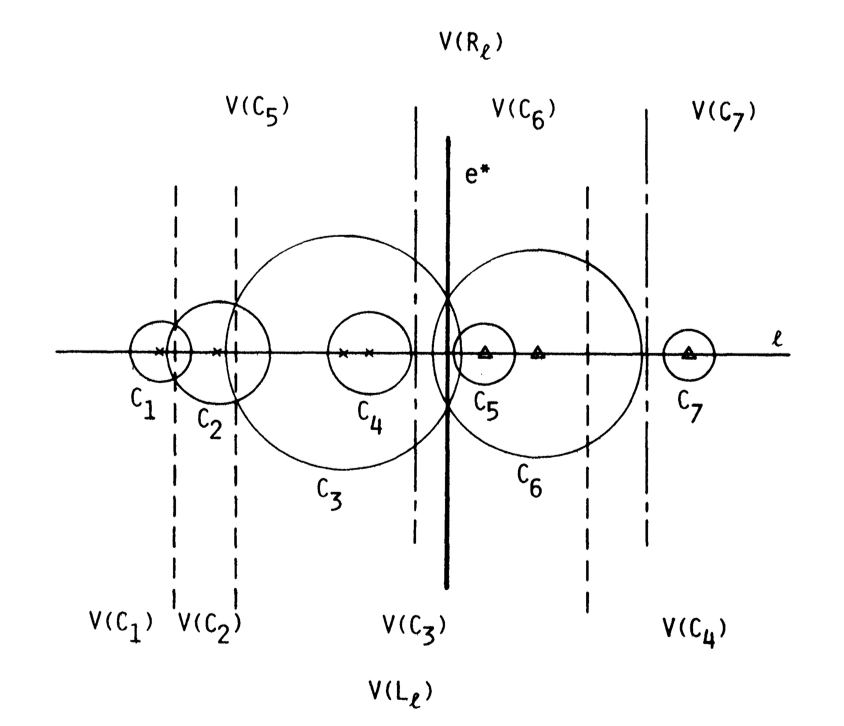
\includegraphics[width=0.5\textwidth]{fig8.png}
    \end{center}
\end{enumerate}

\subsection{延伸應用}
有了上述的演算法,以下兩個問題也能夠在$O(n\log n)$的時間內被以類似的方式求解出來:

\begin{itemize}
    \item \textit{Finding the contour of the union of given $n$ circles} \\    
        可被運用在數據分析。
    \item \textit{Connected components of given $n$ circles} \\
        可被運用在圖片處理及電腦視覺。
\end{itemize}

在這裡我們就不特別詳加敘述此兩問題,因為解法都是建立在沃羅諾伊圖的建構上。

\newpage
\section{閱讀心得}

這次的報告,圖例多了不少,我自認為自己空間觀念薄弱,所以在思考這種跟幾何有關的問題時,總會花上比別人更多的時間。但從此篇東大所著作的論文中,仍然得到滿多收穫的。\\

沃羅諾伊圖在幾何、晶體學、建築學、地理學、氣象學、資訊資統等許多領域都有廣泛的應用。
沃羅諾伊圖在繪製地理資料時,能夠將地圖切成許多分塊,每一塊都有專屬最方便的站點。走在路上,如果想要找間便利商店,我們會打開電子地圖搜尋商店,然後挑一間看起來最近的商店朝著他走去。看似簡單的動作由電腦來做卻不容易;最簡單的做法,是先將所有的便利商店列出來,逐一用當前位置算距離,再取出距離最短的一個。\\

舉例來說,最近台灣空氣汙染嚴重,比如當我們只關心50公里內的空氣汙染指數,那麼我們便以每個可能產生汙染的地點(台中發電廠、通霄發電廠、大潭發電廠等)為圓心建立許多50公里的圓,取沃羅諾伊圖的交集。\\

維諾圖在各個領域的應用還有很多,高效率的演算法都能使得我們在尋找交集求解時,省下大量的時間!
\end{document}